% Options for packages loaded elsewhere
\PassOptionsToPackage{unicode}{hyperref}
\PassOptionsToPackage{hyphens}{url}
%
\documentclass[
]{article}
\usepackage{amsmath,amssymb}
\usepackage{iftex}
\ifPDFTeX
  \usepackage[T1]{fontenc}
  \usepackage[utf8]{inputenc}
  \usepackage{textcomp} % provide euro and other symbols
\else % if luatex or xetex
  \usepackage{unicode-math} % this also loads fontspec
  \defaultfontfeatures{Scale=MatchLowercase}
  \defaultfontfeatures[\rmfamily]{Ligatures=TeX,Scale=1}
\fi
\usepackage{lmodern}
\ifPDFTeX\else
  % xetex/luatex font selection
\fi
% Use upquote if available, for straight quotes in verbatim environments
\IfFileExists{upquote.sty}{\usepackage{upquote}}{}
\IfFileExists{microtype.sty}{% use microtype if available
  \usepackage[]{microtype}
  \UseMicrotypeSet[protrusion]{basicmath} % disable protrusion for tt fonts
}{}
\makeatletter
\@ifundefined{KOMAClassName}{% if non-KOMA class
  \IfFileExists{parskip.sty}{%
    \usepackage{parskip}
  }{% else
    \setlength{\parindent}{0pt}
    \setlength{\parskip}{6pt plus 2pt minus 1pt}}
}{% if KOMA class
  \KOMAoptions{parskip=half}}
\makeatother
\usepackage{xcolor}
\usepackage[margin=1in]{geometry}
\usepackage{color}
\usepackage{fancyvrb}
\newcommand{\VerbBar}{|}
\newcommand{\VERB}{\Verb[commandchars=\\\{\}]}
\DefineVerbatimEnvironment{Highlighting}{Verbatim}{commandchars=\\\{\}}
% Add ',fontsize=\small' for more characters per line
\usepackage{framed}
\definecolor{shadecolor}{RGB}{248,248,248}
\newenvironment{Shaded}{\begin{snugshade}}{\end{snugshade}}
\newcommand{\AlertTok}[1]{\textcolor[rgb]{0.94,0.16,0.16}{#1}}
\newcommand{\AnnotationTok}[1]{\textcolor[rgb]{0.56,0.35,0.01}{\textbf{\textit{#1}}}}
\newcommand{\AttributeTok}[1]{\textcolor[rgb]{0.13,0.29,0.53}{#1}}
\newcommand{\BaseNTok}[1]{\textcolor[rgb]{0.00,0.00,0.81}{#1}}
\newcommand{\BuiltInTok}[1]{#1}
\newcommand{\CharTok}[1]{\textcolor[rgb]{0.31,0.60,0.02}{#1}}
\newcommand{\CommentTok}[1]{\textcolor[rgb]{0.56,0.35,0.01}{\textit{#1}}}
\newcommand{\CommentVarTok}[1]{\textcolor[rgb]{0.56,0.35,0.01}{\textbf{\textit{#1}}}}
\newcommand{\ConstantTok}[1]{\textcolor[rgb]{0.56,0.35,0.01}{#1}}
\newcommand{\ControlFlowTok}[1]{\textcolor[rgb]{0.13,0.29,0.53}{\textbf{#1}}}
\newcommand{\DataTypeTok}[1]{\textcolor[rgb]{0.13,0.29,0.53}{#1}}
\newcommand{\DecValTok}[1]{\textcolor[rgb]{0.00,0.00,0.81}{#1}}
\newcommand{\DocumentationTok}[1]{\textcolor[rgb]{0.56,0.35,0.01}{\textbf{\textit{#1}}}}
\newcommand{\ErrorTok}[1]{\textcolor[rgb]{0.64,0.00,0.00}{\textbf{#1}}}
\newcommand{\ExtensionTok}[1]{#1}
\newcommand{\FloatTok}[1]{\textcolor[rgb]{0.00,0.00,0.81}{#1}}
\newcommand{\FunctionTok}[1]{\textcolor[rgb]{0.13,0.29,0.53}{\textbf{#1}}}
\newcommand{\ImportTok}[1]{#1}
\newcommand{\InformationTok}[1]{\textcolor[rgb]{0.56,0.35,0.01}{\textbf{\textit{#1}}}}
\newcommand{\KeywordTok}[1]{\textcolor[rgb]{0.13,0.29,0.53}{\textbf{#1}}}
\newcommand{\NormalTok}[1]{#1}
\newcommand{\OperatorTok}[1]{\textcolor[rgb]{0.81,0.36,0.00}{\textbf{#1}}}
\newcommand{\OtherTok}[1]{\textcolor[rgb]{0.56,0.35,0.01}{#1}}
\newcommand{\PreprocessorTok}[1]{\textcolor[rgb]{0.56,0.35,0.01}{\textit{#1}}}
\newcommand{\RegionMarkerTok}[1]{#1}
\newcommand{\SpecialCharTok}[1]{\textcolor[rgb]{0.81,0.36,0.00}{\textbf{#1}}}
\newcommand{\SpecialStringTok}[1]{\textcolor[rgb]{0.31,0.60,0.02}{#1}}
\newcommand{\StringTok}[1]{\textcolor[rgb]{0.31,0.60,0.02}{#1}}
\newcommand{\VariableTok}[1]{\textcolor[rgb]{0.00,0.00,0.00}{#1}}
\newcommand{\VerbatimStringTok}[1]{\textcolor[rgb]{0.31,0.60,0.02}{#1}}
\newcommand{\WarningTok}[1]{\textcolor[rgb]{0.56,0.35,0.01}{\textbf{\textit{#1}}}}
\usepackage{graphicx}
\makeatletter
\def\maxwidth{\ifdim\Gin@nat@width>\linewidth\linewidth\else\Gin@nat@width\fi}
\def\maxheight{\ifdim\Gin@nat@height>\textheight\textheight\else\Gin@nat@height\fi}
\makeatother
% Scale images if necessary, so that they will not overflow the page
% margins by default, and it is still possible to overwrite the defaults
% using explicit options in \includegraphics[width, height, ...]{}
\setkeys{Gin}{width=\maxwidth,height=\maxheight,keepaspectratio}
% Set default figure placement to htbp
\makeatletter
\def\fps@figure{htbp}
\makeatother
\setlength{\emergencystretch}{3em} % prevent overfull lines
\providecommand{\tightlist}{%
  \setlength{\itemsep}{0pt}\setlength{\parskip}{0pt}}
\setcounter{secnumdepth}{-\maxdimen} % remove section numbering
\ifLuaTeX
  \usepackage{selnolig}  % disable illegal ligatures
\fi
\IfFileExists{bookmark.sty}{\usepackage{bookmark}}{\usepackage{hyperref}}
\IfFileExists{xurl.sty}{\usepackage{xurl}}{} % add URL line breaks if available
\urlstyle{same}
\hypersetup{
  hidelinks,
  pdfcreator={LaTeX via pandoc}}

\author{}
\date{\vspace{-2.5em}}

\begin{document}

\hypertarget{varying-values-of-parameters}{%
\subsubsection{Varying values of
parameters}\label{varying-values-of-parameters}}

\begin{enumerate}
\def\labelenumi{\arabic{enumi}.}
\tightlist
\item
  \(G(v) = v^\kappa, \ \kappa > 0\)
  \[F_1(x) = \{1 - [1 + \xi(\frac{x}{\sigma})]^{-1/\xi} \}^\kappa\]
  \[f_1(x) = \frac{\kappa}{\sigma}[1 + \xi (\frac{x}{\sigma})]^{-(1/\xi + 1)}\{1 - [1+\xi(\frac{x}{\sigma})]^{-1/\xi} \} ^{\kappa-1}\]
\end{enumerate}

\(\kappa\) varying: pdf

\begin{Shaded}
\begin{Highlighting}[]
\FunctionTok{curve}\NormalTok{(}\FunctionTok{g1\_pdf}\NormalTok{(x, }\AttributeTok{sigma =} \DecValTok{1}\NormalTok{, }\AttributeTok{xi =} \FloatTok{0.5}\NormalTok{, }\AttributeTok{kappa =} \DecValTok{1}\NormalTok{), }\AttributeTok{xlim =} \FunctionTok{c}\NormalTok{(}\DecValTok{0}\NormalTok{, }\FloatTok{7.5}\NormalTok{))}
\FunctionTok{curve}\NormalTok{(}\FunctionTok{g1\_pdf}\NormalTok{(x, }\AttributeTok{sigma =} \DecValTok{1}\NormalTok{, }\AttributeTok{xi =} \FloatTok{0.5}\NormalTok{, }\AttributeTok{kappa =} \DecValTok{2}\NormalTok{), }\AttributeTok{xlim =} \FunctionTok{c}\NormalTok{(}\DecValTok{0}\NormalTok{, }\FloatTok{7.5}\NormalTok{), }\AttributeTok{add =} \ConstantTok{TRUE}\NormalTok{, }\AttributeTok{col =} \StringTok{\textquotesingle{}blue\textquotesingle{}}\NormalTok{)}
\FunctionTok{curve}\NormalTok{(}\FunctionTok{g1\_pdf}\NormalTok{(x, }\AttributeTok{sigma =} \DecValTok{1}\NormalTok{, }\AttributeTok{xi =} \FloatTok{0.5}\NormalTok{, }\AttributeTok{kappa =} \DecValTok{5}\NormalTok{), }\AttributeTok{xlim =} \FunctionTok{c}\NormalTok{(}\DecValTok{0}\NormalTok{, }\FloatTok{7.5}\NormalTok{), }\AttributeTok{add =} \ConstantTok{TRUE}\NormalTok{, }\AttributeTok{col =} \StringTok{\textquotesingle{}red\textquotesingle{}}\NormalTok{)}
\FunctionTok{curve}\NormalTok{(}\FunctionTok{g1\_pdf}\NormalTok{(x, }\AttributeTok{sigma =} \DecValTok{1}\NormalTok{, }\AttributeTok{xi =} \FloatTok{0.5}\NormalTok{, }\AttributeTok{kappa =} \DecValTok{8}\NormalTok{), }\AttributeTok{xlim =} \FunctionTok{c}\NormalTok{(}\DecValTok{0}\NormalTok{, }\FloatTok{7.5}\NormalTok{), }\AttributeTok{add =} \ConstantTok{TRUE}\NormalTok{, }\AttributeTok{col =} \StringTok{\textquotesingle{}green\textquotesingle{}}\NormalTok{)}
\end{Highlighting}
\end{Shaded}

\begin{center}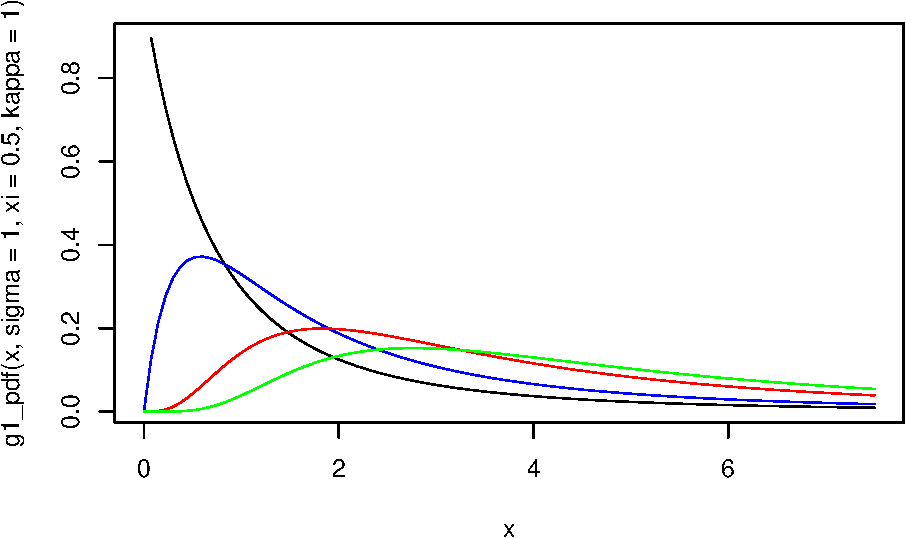
\includegraphics[width=0.8\linewidth]{g1_varying_params_files/figure-latex/unnamed-chunk-2-1} \end{center}

\(\kappa\) varying: cdf

\begin{center}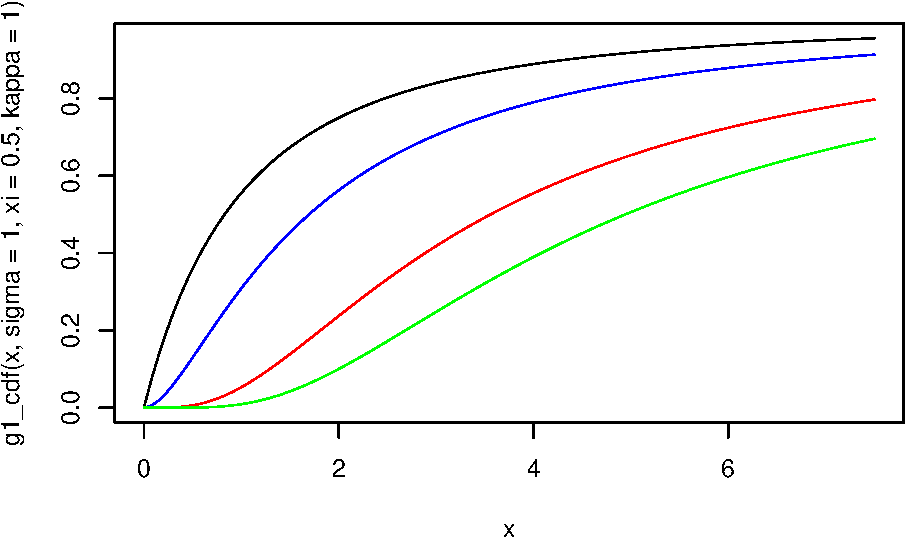
\includegraphics[width=0.8\linewidth]{g1_varying_params_files/figure-latex/unnamed-chunk-3-1} \end{center}
\pagebreak

\(\sigma\) varying: pdf

\begin{Shaded}
\begin{Highlighting}[]
\FunctionTok{curve}\NormalTok{(}\FunctionTok{g1\_pdf}\NormalTok{(x, }\AttributeTok{sigma =} \DecValTok{1}\NormalTok{, }\AttributeTok{xi =} \FloatTok{0.5}\NormalTok{, }\AttributeTok{kappa =} \DecValTok{1}\NormalTok{), }\AttributeTok{xlim =} \FunctionTok{c}\NormalTok{(}\DecValTok{0}\NormalTok{, }\FloatTok{7.5}\NormalTok{))}
\FunctionTok{curve}\NormalTok{(}\FunctionTok{g1\_pdf}\NormalTok{(x, }\AttributeTok{sigma =} \DecValTok{2}\NormalTok{, }\AttributeTok{xi =} \FloatTok{0.5}\NormalTok{, }\AttributeTok{kappa =} \DecValTok{1}\NormalTok{), }\AttributeTok{xlim =} \FunctionTok{c}\NormalTok{(}\DecValTok{0}\NormalTok{, }\FloatTok{7.5}\NormalTok{), }\AttributeTok{add =} \ConstantTok{TRUE}\NormalTok{, }\AttributeTok{col =} \StringTok{\textquotesingle{}blue\textquotesingle{}}\NormalTok{)}
\FunctionTok{curve}\NormalTok{(}\FunctionTok{g1\_pdf}\NormalTok{(x, }\AttributeTok{sigma =} \DecValTok{4}\NormalTok{, }\AttributeTok{xi =} \FloatTok{0.5}\NormalTok{, }\AttributeTok{kappa =} \DecValTok{1}\NormalTok{), }\AttributeTok{xlim =} \FunctionTok{c}\NormalTok{(}\DecValTok{0}\NormalTok{, }\FloatTok{7.5}\NormalTok{), }\AttributeTok{add =} \ConstantTok{TRUE}\NormalTok{, }\AttributeTok{col =} \StringTok{\textquotesingle{}red\textquotesingle{}}\NormalTok{)}
\FunctionTok{curve}\NormalTok{(}\FunctionTok{g1\_pdf}\NormalTok{(x, }\AttributeTok{sigma =} \DecValTok{6}\NormalTok{, }\AttributeTok{xi =} \FloatTok{0.5}\NormalTok{, }\AttributeTok{kappa =} \DecValTok{1}\NormalTok{), }\AttributeTok{xlim =} \FunctionTok{c}\NormalTok{(}\DecValTok{0}\NormalTok{, }\FloatTok{7.5}\NormalTok{), }\AttributeTok{add =} \ConstantTok{TRUE}\NormalTok{, }\AttributeTok{col =} \StringTok{\textquotesingle{}green\textquotesingle{}}\NormalTok{)}
\end{Highlighting}
\end{Shaded}

\begin{center}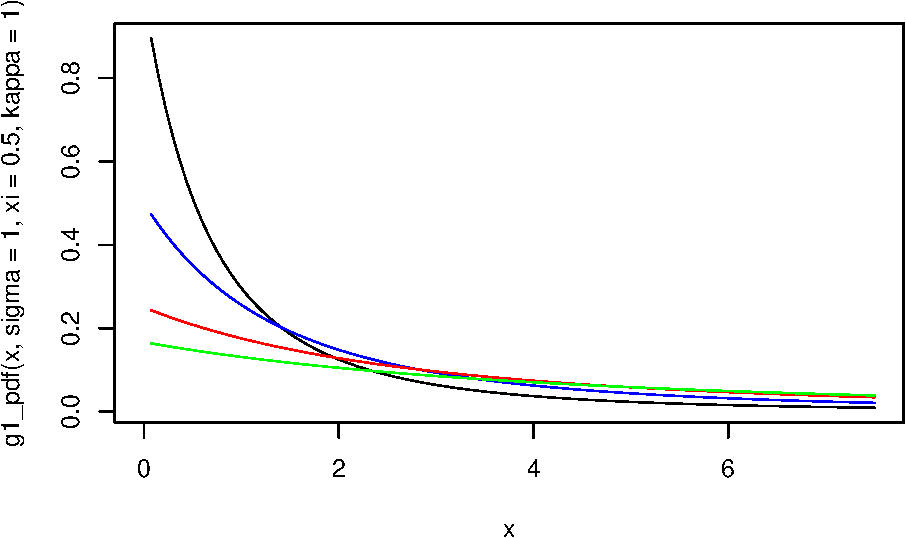
\includegraphics[width=0.8\linewidth]{g1_varying_params_files/figure-latex/unnamed-chunk-4-1} \end{center}

\(\sigma\) varying: cdf

\begin{Shaded}
\begin{Highlighting}[]
\FunctionTok{curve}\NormalTok{(}\FunctionTok{g1\_cdf}\NormalTok{(x, }\AttributeTok{sigma =} \DecValTok{1}\NormalTok{, }\AttributeTok{xi =} \FloatTok{0.5}\NormalTok{, }\AttributeTok{kappa =} \DecValTok{1}\NormalTok{), }\AttributeTok{xlim =} \FunctionTok{c}\NormalTok{(}\DecValTok{0}\NormalTok{, }\FloatTok{7.5}\NormalTok{))}
\FunctionTok{curve}\NormalTok{(}\FunctionTok{g1\_cdf}\NormalTok{(x, }\AttributeTok{sigma =} \DecValTok{2}\NormalTok{, }\AttributeTok{xi =} \FloatTok{0.5}\NormalTok{, }\AttributeTok{kappa =} \DecValTok{1}\NormalTok{), }\AttributeTok{xlim =} \FunctionTok{c}\NormalTok{(}\DecValTok{0}\NormalTok{, }\FloatTok{7.5}\NormalTok{), }\AttributeTok{add =} \ConstantTok{TRUE}\NormalTok{, }\AttributeTok{col =} \StringTok{\textquotesingle{}blue\textquotesingle{}}\NormalTok{)}
\FunctionTok{curve}\NormalTok{(}\FunctionTok{g1\_cdf}\NormalTok{(x, }\AttributeTok{sigma =} \DecValTok{4}\NormalTok{, }\AttributeTok{xi =} \FloatTok{0.5}\NormalTok{, }\AttributeTok{kappa =} \DecValTok{1}\NormalTok{), }\AttributeTok{xlim =} \FunctionTok{c}\NormalTok{(}\DecValTok{0}\NormalTok{, }\FloatTok{7.5}\NormalTok{), }\AttributeTok{add =} \ConstantTok{TRUE}\NormalTok{, }\AttributeTok{col =} \StringTok{\textquotesingle{}red\textquotesingle{}}\NormalTok{)}
\FunctionTok{curve}\NormalTok{(}\FunctionTok{g1\_cdf}\NormalTok{(x, }\AttributeTok{sigma =} \DecValTok{6}\NormalTok{, }\AttributeTok{xi =} \FloatTok{0.5}\NormalTok{, }\AttributeTok{kappa =} \DecValTok{1}\NormalTok{), }\AttributeTok{xlim =} \FunctionTok{c}\NormalTok{(}\DecValTok{0}\NormalTok{, }\FloatTok{7.5}\NormalTok{), }\AttributeTok{add =} \ConstantTok{TRUE}\NormalTok{, }\AttributeTok{col =} \StringTok{\textquotesingle{}green\textquotesingle{}}\NormalTok{)}
\end{Highlighting}
\end{Shaded}

\begin{center}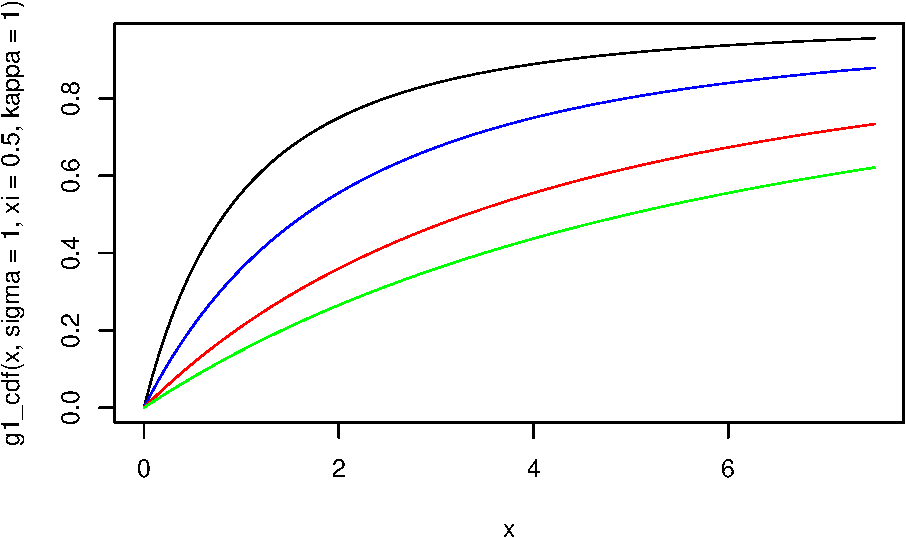
\includegraphics[width=0.8\linewidth]{g1_varying_params_files/figure-latex/unnamed-chunk-5-1} \end{center}
\pagebreak

\(\xi\) varying: pdf

\begin{Shaded}
\begin{Highlighting}[]
\FunctionTok{curve}\NormalTok{(}\FunctionTok{g1\_pdf}\NormalTok{(x, }\AttributeTok{sigma =} \DecValTok{1}\NormalTok{, }\AttributeTok{xi =} \FloatTok{0.25}\NormalTok{, }\AttributeTok{kappa =} \DecValTok{1}\NormalTok{), }\AttributeTok{xlim =} \FunctionTok{c}\NormalTok{(}\DecValTok{0}\NormalTok{, }\FloatTok{7.5}\NormalTok{))}
\FunctionTok{curve}\NormalTok{(}\FunctionTok{g1\_pdf}\NormalTok{(x, }\AttributeTok{sigma =} \DecValTok{1}\NormalTok{, }\AttributeTok{xi =} \FloatTok{0.5}\NormalTok{, }\AttributeTok{kappa =} \DecValTok{1}\NormalTok{), }\AttributeTok{xlim =} \FunctionTok{c}\NormalTok{(}\DecValTok{0}\NormalTok{, }\FloatTok{7.5}\NormalTok{), }\AttributeTok{add =} \ConstantTok{TRUE}\NormalTok{, }\AttributeTok{col =} \StringTok{\textquotesingle{}blue\textquotesingle{}}\NormalTok{)}
\FunctionTok{curve}\NormalTok{(}\FunctionTok{g1\_pdf}\NormalTok{(x, }\AttributeTok{sigma =} \DecValTok{1}\NormalTok{, }\AttributeTok{xi =} \FloatTok{0.75}\NormalTok{, }\AttributeTok{kappa =} \DecValTok{1}\NormalTok{), }\AttributeTok{xlim =} \FunctionTok{c}\NormalTok{(}\DecValTok{0}\NormalTok{, }\FloatTok{7.5}\NormalTok{), }\AttributeTok{add =} \ConstantTok{TRUE}\NormalTok{, }\AttributeTok{col =} \StringTok{\textquotesingle{}red\textquotesingle{}}\NormalTok{)}
\FunctionTok{curve}\NormalTok{(}\FunctionTok{g1\_pdf}\NormalTok{(x, }\AttributeTok{sigma =} \DecValTok{1}\NormalTok{, }\AttributeTok{xi =} \DecValTok{1}\NormalTok{, }\AttributeTok{kappa =} \DecValTok{1}\NormalTok{), }\AttributeTok{xlim =} \FunctionTok{c}\NormalTok{(}\DecValTok{0}\NormalTok{, }\FloatTok{7.5}\NormalTok{), }\AttributeTok{add =} \ConstantTok{TRUE}\NormalTok{, }\AttributeTok{col =} \StringTok{\textquotesingle{}green\textquotesingle{}}\NormalTok{)}
\end{Highlighting}
\end{Shaded}

\begin{center}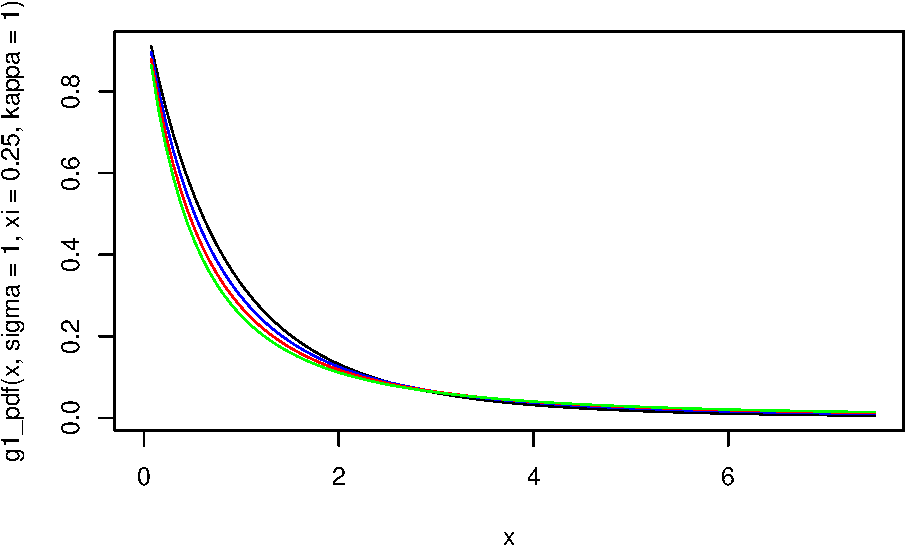
\includegraphics[width=0.8\linewidth]{g1_varying_params_files/figure-latex/unnamed-chunk-6-1} \end{center}

\(\xi\) varying: cdf

\begin{Shaded}
\begin{Highlighting}[]
\FunctionTok{curve}\NormalTok{(}\FunctionTok{g1\_cdf}\NormalTok{(x, }\AttributeTok{sigma =} \DecValTok{1}\NormalTok{, }\AttributeTok{xi =} \FloatTok{0.25}\NormalTok{, }\AttributeTok{kappa =} \DecValTok{1}\NormalTok{), }\AttributeTok{xlim =} \FunctionTok{c}\NormalTok{(}\DecValTok{0}\NormalTok{, }\FloatTok{7.5}\NormalTok{))}
\FunctionTok{curve}\NormalTok{(}\FunctionTok{g1\_cdf}\NormalTok{(x, }\AttributeTok{sigma =} \DecValTok{1}\NormalTok{, }\AttributeTok{xi =} \FloatTok{0.5}\NormalTok{, }\AttributeTok{kappa =} \DecValTok{1}\NormalTok{), }\AttributeTok{xlim =} \FunctionTok{c}\NormalTok{(}\DecValTok{0}\NormalTok{, }\FloatTok{7.5}\NormalTok{), }\AttributeTok{add =} \ConstantTok{TRUE}\NormalTok{, }\AttributeTok{col =} \StringTok{\textquotesingle{}blue\textquotesingle{}}\NormalTok{)}
\FunctionTok{curve}\NormalTok{(}\FunctionTok{g1\_cdf}\NormalTok{(x, }\AttributeTok{sigma =} \DecValTok{1}\NormalTok{, }\AttributeTok{xi =} \FloatTok{0.75}\NormalTok{, }\AttributeTok{kappa =} \DecValTok{1}\NormalTok{), }\AttributeTok{xlim =} \FunctionTok{c}\NormalTok{(}\DecValTok{0}\NormalTok{, }\FloatTok{7.5}\NormalTok{), }\AttributeTok{add =} \ConstantTok{TRUE}\NormalTok{, }\AttributeTok{col =} \StringTok{\textquotesingle{}red\textquotesingle{}}\NormalTok{)}
\FunctionTok{curve}\NormalTok{(}\FunctionTok{g1\_cdf}\NormalTok{(x, }\AttributeTok{sigma =} \DecValTok{1}\NormalTok{, }\AttributeTok{xi =} \DecValTok{1}\NormalTok{, }\AttributeTok{kappa =} \DecValTok{1}\NormalTok{), }\AttributeTok{xlim =} \FunctionTok{c}\NormalTok{(}\DecValTok{0}\NormalTok{, }\FloatTok{7.5}\NormalTok{), }\AttributeTok{add =} \ConstantTok{TRUE}\NormalTok{, }\AttributeTok{col =} \StringTok{\textquotesingle{}green\textquotesingle{}}\NormalTok{)}
\end{Highlighting}
\end{Shaded}

\begin{center}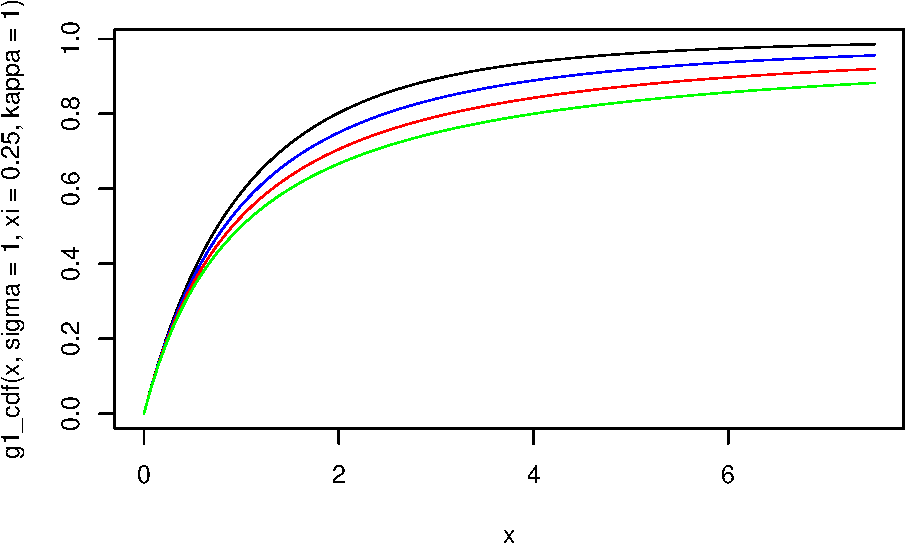
\includegraphics[width=0.8\linewidth]{g1_varying_params_files/figure-latex/unnamed-chunk-7-1} \end{center}

\end{document}
